\chapter{Introduction et plan d'intégration}
\chaptermark{Intro}
\section{Présentation du problème} 
Ce TP évalué a pour objectif de corriger un logiciel de jeu d'échecs codé en java.  

\section{Plan d'intégration}
Le logiciel utilisait le design pattern MVC. Il était demandé de se focaliser sur la partie métier uniquement. A l'origine nous dispostion du document suivant créer notre plan d'intégration : 
   \begin{figure}[htbp]
  \centering
  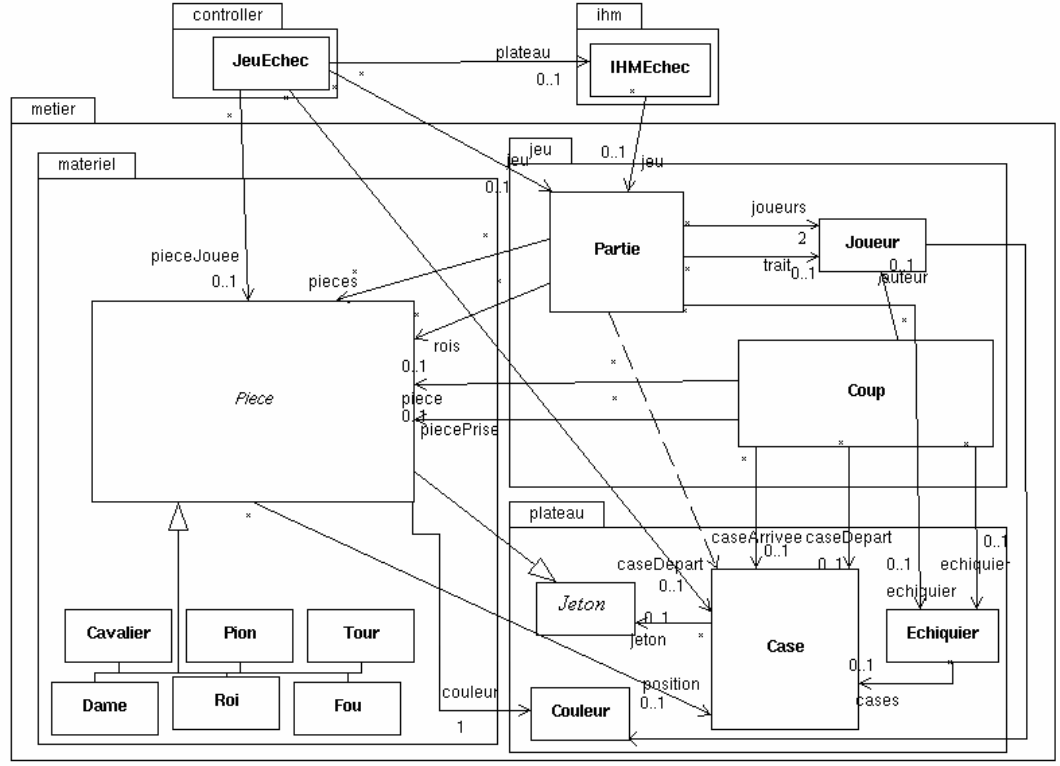
\includegraphics[scale=0.39]{img/uml}
  \caption{Diagramme UML de la partie métier}
  \label{fig:uml}
\end{figure}
\clearpage

Au terme de notre réflexion nous avons obtenu le graphe de dépendances  suivant : 
   \begin{figure}[htbp]
  \centering
  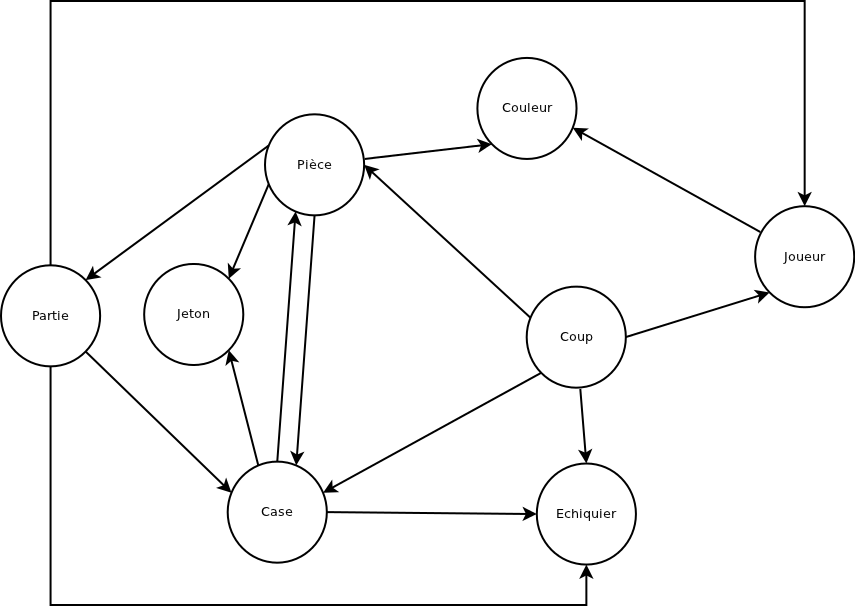
\includegraphics[scale=0.40]{img/PlanI}
  \caption{Graphe de dépendance}
  \label{fig:GDT}
\end{figure}

Le plan d'intégration en utilisant un stub de la classe de Case découle du graph de dépendances à savoir : 
\begin{itemize}
\item
Couleur (Ne dépend de rien)
\item
Joueur (Dépend de couleur)
\end{itemize}

Puis : 

\begin{itemize}
\item
Pièce(Avec StubCase)
\item
Echiquier(Avec StubCase)
\item
Coups(Avec StubCase)
\item
Partie(Avec StubCase)
\item
Case
\item
Pièce
\item
Echiquier
\item
Coup
\item
Partie
\end{itemize}

